\documentclass[10pt]{article}
\usepackage[dvipsnames]{xcolor}
\usepackage{tikz}
\usepackage{url}
\usepackage{multicol}
\usepackage{xspace}
\usepackage{pstricks}
\usepackage{wrapfig}
\usepackage[section]{placeins}
\usepackage{wrapfig}
\usepackage[default]{droidserif}
\usepackage[T1]{fontenc}
\usepackage{listings}
%\usepackage{algorithm2e}
\usetikzlibrary{arrows,automata,shapes}
\tikzstyle{block} = [rectangle, draw, fill=blue!20,
text width=2.5em, text centered, rounded corners, minimum height=2em]
\tikzstyle{bw} = [rectangle, draw, fill=blue!20,
text width=4em, text centered, rounded corners, minimum height=2em]
\newcommand{\handout}[5]{
\noindent
\begin{center}
\framebox{
\vbox{
\hbox to 5.78in { {\bf ECE155: Engineering Design with Embedded Systems } \hfill #2 }
\vspace{4mm}
\hbox to 5.78in { {\Large \hfill #5 \hfill} }
\vspace{2mm}
\hbox to 5.78in { {\em #3 \hfill #4} }
}
}
\end{center}
\vspace*{4mm}
}
\newcommand{\lecture}[4]{\handout{#1}{#2}{#3}{#4}{Lab #1}}
\topmargin 0pt
\advance \topmargin by -\headheight
\advance \topmargin by -\headsep
\textheight 8.9in
\oddsidemargin 0pt
\evensidemargin \oddsidemargin
\marginparwidth 0.5in
\textwidth 6.5in
\parindent 0in
\parskip 1.5ex
%\renewcommand{\baselinestretch}{1.25}
\newcommand{\todo}[1]{{\red\textbf{TODO: }#1}\xspace}
\lstset{language=java,
basicstyle=\ttfamily,columns=fullflexible,
% keywordstyle=\color{Blue}, % keyword style
% commentstyle=\color{OliveGreen}\textit, % comment style
% identifierstyle=\color{Black},
% stringstyle=\color{BrickRed},
mathescape=true,
tabsize=3,
showstringspaces=false}
\begin{document}
\lecture{1 (Reading Sensors \& The Android API)}{Winter 2015}{Prepared by Kirill Morozov, Han Xu, Zheng Ma, Devin Binnie}{version 1.5}
{ \bf Deadline:} You must submit the lab to the SVN repository by the submission deadline (see the syllabus) and be
prepared to demonstrate Lab 1 to a TA at the start of your assigned
Lab 2 session. The best way to demo is during a lab session, but any
earlier time where you can convince a TA to watch is OK too.
\section{Objective}
The objectives of Lab 1 are for you to:
\begin{enumerate}
\item Familiarize yourself with the Android phones that you will be developing for, and
\item Learn how to read the sensors on these phones.
\end{enumerate}
During this lab, you will write a simple Android application that reads the various sensors available on the phone and graphs them. Your code will initialize an Android Activity; accept the values from the phone's sensors; and display these values on the screen. Consult the lecture notes \& slides for more details on what Android Activities are.
The steps in this lab will be:
\begin{enumerate}
\item Use the Eclipse IDE and the Android API to create a basic Android application.
\item Add items to the user interface for your Android application.
\item Create event handlers for a variety of sensors and make them modify the user interface.
\item Include a widget to graph a history of sensor values.
\end{enumerate}
\paragraph{Deliverables.} For this lab, you must:
\begin{itemize}
\item Create a system that will let you display each sensor's current value when the event is received using an event handler. (See Figure~\ref{fig:device-screenshot}, field ``Acceleration (linear) ($m/s^2$)''.)
\item Since the reading from the sensors will change quickly, you must also display the all-time highest or lowest (depending on which is greater in absolute value) readings from each sensor so that we can see concrete numbers. (Field ``Record Acceleration (linear) ($m/s^2$)'' in Figure~\ref{fig:device-screenshot}.)
%\item stop the phone from reorienting its screen when you rotate it.
\item Ensure that the data you display is readable, accessible to the user, and that it does not vanish off the edge of the screen. How you do this is up to you. For instance, you can enable scrolling, or simply format the data effectively. Any functional system is acceptable.
\end{itemize}
%\todo{include an example; include hints on how to do this; how much data do we want exactly}
%\begin{wrapfigure} {R}{0.5\textwidth}
\begin{figure}[htbp]
\begin{center}
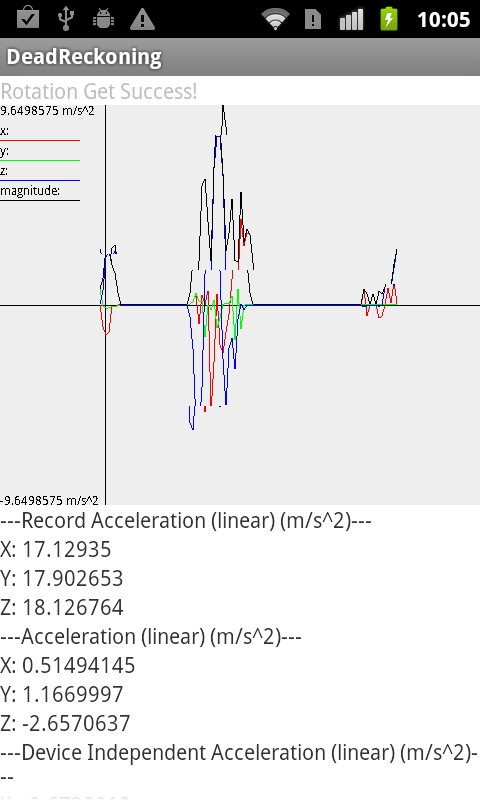
\includegraphics[height=20em]{device-screenshot.png}
\end{center}
\caption{\label{fig:device-screenshot}An example of a completed Lab 1.}
\end{figure}
%\vspace{-50pt}
%\end{wrapfigure}
\section{Phases of the lab}
The recommended procedure to complete the lab is as follows:
\begin{enumerate}
\item Create infrastructure to display raw data to the user.
\item Create handlers to read and record sensor values.
%% \item Create a system to transfer the collected data from the phone to your computer.
\item Test.
\item Demonstrate.
\end{enumerate}
\section{Create infrastructure to display data to the user}
Before we continue, we'll explain the structure of an Android application and about JavaDoc.
\subsection{Digression 1: About the Android application structure}
Even the empty Android project (e.g. from Lab 0) contains folders and files. Here's what they do.
\begin{itemize}
\item The ``{\tt src}'' folder contains all of your {\tt .java} files for the project. Here you will add the code you'll write. The empty project already contains a ``Hello World'' activity, {\tt MainActivity}.
\item The ``{\tt gen}'' folder contains automatically generated {\tt .java} files. Of particular interest is the {\tt R.java} file which mirrors the constants and ids you will define in the project's xml. \emph{Do not edit these files directly. Your changes will be lost when you build your code next.}
\item The ``{\tt bin}'' folder is the output directory for the project. Compiled files appear here.
\item The ``{\tt libs}'' folder contains your private libraries. (You can ignore this.)
\item The ``{\tt res}'' folder contains application resources, such as drawable files, layout files, and string values. The ``{\tt res/layout}'' folder is important. Each xml file in that folder describes the layout of controls in a single activity in your application. %The Eclipse plug-in provides a graphical editor for this layout. Unfortunately, it is not very good. You are going to have an easier time editing these xml files by hand.
\end{itemize}
\paragraph{About Activities.}
The fundamental building block of an Android application is the ``Activity.'' Activities represent screens in your application. When a screen gains focus, Android activates the appropriate activity, which may then interact with the user. When the user switches to a different screen, Android disables the activity, preserving the program state.
The new Android application wizard will create a blank \texttt{MainActivity} for you. You can work exclusively with that activity, and you won't need to create any new activities for these labs.
%% If you do create additional activities, you can launch them in one of three ways:
%% \begin{itemize}
%% \item Change the starting activity by clicking the drop-down arrow beside the run button and select \textbf{Run configurations...} and then change the launch action to launch the specific activity you want.
%% \item Edit the {\tt AndroidManifest.xml} file. On the Application tab, you will find a sub-window called \textbf{Application Nodes}. The activity at the top of that list is the default activity; it will be launched first.
%% \item Launch the activity programmatically by calling {\tt Context.startActivity()};
%% \end{itemize}
\paragraph{Random testing-related tip.} If you did not change anything in your code since the last time you launched your application, Eclipse will not re-upload or restart your application when you click \textbf{Run}. Instead, it will just make your application active again. If you are trying to reset your application's state, you will either need to build that option in yourself, or force Eclipse to recompile your application.
\subsection{Digression 2: Helping you help yourself: On JavaDoc} For the next step, the rest of the labs, and life in general, you need to learn how to navigate JavaDocs. JavaDoc is documentation automatically extracted from Java programs---while these programs were being developed, developers and technical writers added JavaDoc documentation in the form of specially formatted comments in their source code.
Android's JavaDoc documentation is thorough and easy to read. It is at \url{http://developer.android.com/reference/packages.html}. If you installed the documentation when you installed the Android SDK, you can also reach the documentation from Eclipse. To do this, hover the mouse over something that you want documentation about. A yellow box will pop up; click on it. Finally, click the right-most button that appears at the bottom of this box. See figure \ref{fig:javadoc-tooltip} for an example. Keep in mind that you can only hover over something that is defined by the Android SDK. If you try to hover over one of your own classes or variables, Eclipse will look for the JavaDoc attached to your code, and will not find it (unless you add it yourself.)
\begin{figure}[ht]
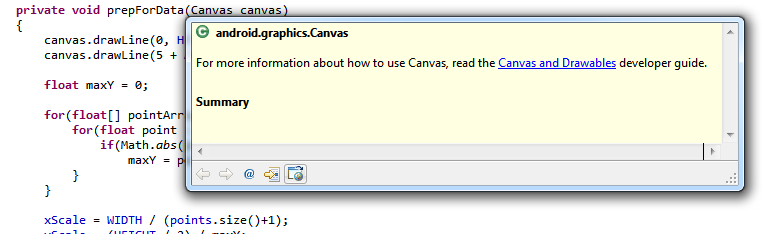
\includegraphics[width=\textwidth]{Javadoc-tooltip.png}
\caption{\label{fig:javadoc-tooltip}Tool-tip you'll see when mousing over a class name.}
\end{figure}
\subsection{Back to displaying data to the user} The immediate goal of this exercise is to display information to the user. The best way to do that is by creating labels and modifying their contents programmatically. We'll walk you through changing the content of the ``Hello World'' label from Lab 0.
The Main activity contains the ``Hello World'' label. To reference this label from your code, you need to give it an ID (identifier). Or, in other words, we need a way to refer to that label. Here's how.
\begin{enumerate}
\item Create a new Android project and in the "Create Activity" window choose "Blank Activity with fragment".
\item Open the fragment\_main.xml file located in \textbf{[your project] \textgreater~res \textgreater~layout}.
\item Switch to the xml tab at the bottom of the editor.
\item Look for the xml tag \verb+<TextView>+ and add the attribute \verb-android:id="@+id/label1"-.
\end{enumerate}
In the Android API, all user-visible controls are sub-classes of {\tt android.view.View}. You can get a reference to the ``Hello World'' label by calling {\tt findViewById()} in your Activity with the label id (which you just added) as a parameter. The return value of this function will be the View object that has the ID provided as an argument to the function. The Android compilation system will add the ids to the {\tt R} class. For instance, to find the label you just added above, you might call {\tt findViewById(R.id.label1)}.
Labels are {\tt TextView} objects. You can change the text of a label by calling {\tt TextView.setText()}. You can just pass any {\tt String} to
{\tt TextView.setText()}, and Android will automatically redraw the label with the
new value.
In particular, here's how to modify the ``Hello World'' label, after you've followed
the steps above.
\begin{enumerate}
\item Open {\tt MainActivity.java} in \textbf{[your project] \textgreater~src \textgreater~ca.uwaterloo.[your project]}.
\item Write the following {\tt PlaceholderFragment()} class:
\begin{lstlisting}[]{}
public static class PlaceholderFragment extends Fragment {
public PlaceholderFragment() {
}
@Override
public View onCreateView(LayoutInflater inflater, ViewGroup container,
Bundle savedInstanceState) {
View rootView = inflater.inflate(R.layout.fragment_main, container,
false);
TextView tv = (TextView) rootView.findViewById(R.id.label1);
tv.setText("I've replaced the label!");
return rootView;
}
}
\end{lstlisting}
\end{enumerate}
\paragraph{Non-deliverable.} You should now have an Android application where you can change the label. We are, however, going to take a step back and remove that label, replacing it with automatically-generated labels.
\subsection{Adding more labels}
You'll need to create additional labels to display all the needed data. Of course, you could do this ``by hand'': modify the layout xml for your activity directly, or use the graphical layout tool (double-click on the layout xml). This lab requires creating a lot of labels, and doing that by hand is tedious. Engineers ruthlessly automate. Conveniently, the Android API lets you create views programmatically. Here's how to create one label and add it to a view. First, assign an id to the parent:
\begin{enumerate}
\item In the layout XML, find the \texttt{<RelativeLayout>} tag and assign it an id like you did the label.
\item In the \texttt{onCreateView()} method of the \texttt{PlaceHolderFragment} class, declare and initialize a new \texttt{TextView} object as follows:\\
\texttt{TextView tv1 = new TextView(rootView.getContext());}
\item Then, set the text as above: \texttt{tv1.setText("Example Text");}
\item In the \texttt{onCreateView()} method of your \texttt{PlaceholderFragment} class, get a reference to the \texttt{RelativeView} object that we assigned an id to by using \texttt{findViewByID()}.
\item Add the \texttt{TextView} to the layout by using the \texttt{addView()} method:
\texttt{layout.addView(tv1)}
\item Repeat steps 2 through 5 as necessary to add more labels as needed.
\end{enumerate}
Then, in your PlaceholderFragment's {\tt onCreateView()} method:
\begin{enumerate}
\item Get a reference to the top-level layout (which you just assigned an id to) by using \texttt{findViewByIdwith} the parameter of the ID of the layout (usually starts with \texttt{R.id.}. Cast the result to \texttt{RelativeLayout}.
\item Create a new \texttt{TextView}, e.g. \texttt{TextView tv1 = new TextView(rootView.getContext())}
\item Set the text of \texttt{tv1}, as above.
\item Add \texttt{tv1} to the layout by calling \texttt{addView(tv1)} on the top-level layout.
\end{enumerate}
You can do this several times. You will find that you can save some effort if you write a method to create a new label, add it to the layout and return a reference to the new label.
\paragraph{Common Problems}
At this stage or very soon afterwards, you'll need to create member variables to contain your {\tt TextViews}. You can not call {\tt getApplicationContext()} or {\tt findViewById()} before the {\tt onCreate()} method is executed. For example, the following will cause an null pointer exception:
\begin{verbatim}
public class MyActivity extends ActionBarActivity {
TextView globalView = new TextView(getApplicationContext()); // Error
TextView anotherGlobalView = findViewById(R.id.view1); // Another Error
}
\end{verbatim} \vspace*{-1em}
Do this instead:
\begin{verbatim}
public class MyActivity extends ActionBarActivity {
public View onCreateView(LayoutInflater inflater, ViewGroup container,
Bundle savedInstanceState) {
LinearLayout lmain = (LinearLayout) rootView.findViewById(R.id.Label1);
TextView tv1 = new TextView(rootView.getContext());
tv1.setText(``Example'');
lmain.addView(tv1);
return rootView;
}
}
\end{verbatim} \vspace*{-1em}
\paragraph{RelativeLayout versus LinearLayout.} You'll find
that after you follow the above directions and add a number of labels, your {\tt TextView}s all run into each other. It is possible to configure the {\tt TextView} objects to not step over each other. But it's easier to change {\tt RelativeLayout} for {\tt LinearLayout}, which automatically puts its contents in non-overlapping positions.
\begin{enumerate}
\item In {\tt frament\_main.xml}, change {\tt RelativeLayout} to {\tt LinearLayout}. You have to do that in both the \verb+<RelativeLayout>+ and \verb+</RelativeLayout>+ tags.
\item In {\tt MainActivity.java}, change the line \vspace*{-1em}
\begin{verbatim}
RelativeLayout l = (RelativeLayout)findViewById(R.id.fragment_main);
\end{verbatim} \vspace*{-1em}
to
\vspace*{-1em} \begin{verbatim}
LinearLayout l = (LinearLayout)findViewById(R.id.fragment_main);
\end{verbatim}
\item Add the line \vspace*{-1em}
\begin{verbatim}
l.setOrientation(LinearLayout.VERTICAL);
\end{verbatim} \vspace*{-1em}
which will stack all of the {\tt TextView} objects vertically rather than horizontally.
\end{enumerate}
\paragraph{Deliverable.} Add labels for all of the sensors that we'll record in the next stage. Your Android app should now have a number of labels on the screen, which you should have created programmatically. But you might be displaying more labels than will fit on the screen.
\subsection{Scrolling}
It is easy to implement a scrollbar so that the user can look at all of the labels that you've added. This will not be necessary on a device with a sufficiently-sized screen, but not all devices are large.
\begin{enumerate}
\item Go back to {\tt fragment\_main.xml}, where you should currently have a top-level {\tt LinearLayout}. Before the {\tt LinearLayout}, introduce a {\tt ScrollView}:
\begin{lstlisting}
<ScrollView xmlns:android="http://schemas.android.com/apk/res/android"
android:id="@+id/scroll" android:layout_width="fill_parent"
android:layout_height="wrap_content">
\end{lstlisting}
and close the tag after the {\tt LinearLayout}:
\begin{lstlisting}
</ScrollView>
\end{lstlisting}
\item Change the attribute \verb+android:layout_height+'s value from \verb+match_parent+ to \verb+wrap_content+.
\item Notice that remember to move two \texttt{xmlns} attributes inside \texttt{LinearLayout} to the beginning of \texttt{ScrollView} tag. And delete the repeated line. 
\item Select all codes in \verb+fragment_main.xml+ and press \texttt{<ctrl+i>} to modify the indentation. 
\end{enumerate}
\paragraph{Deliverable.} If you have more content than fits on the screen, make sure that all of the content is somehow viewable.
\section{Create handlers to read and record sensor values}
\paragraph{Tip.} You saw the C\# syntax {\tt String.Format} in ECE150. The corresponding Java syntax is:
\begin{verbatim}
String s = String.format("(%f, %f, %f)", x, y, z);
\end{verbatim}
This will allow you to display $(x, y, z)$ coordinate triples, which will be helpful. You may also want to not display 6 decimal places. I'll leave figuring out how to do that up to you. Use the Internet.
Now that you can display data to the user, you need some data to display. For this lab, you'll need to get that data from the phone's sensors. A number of Android classes collaborate to allow you to read this data, including:
\begin{itemize}
\item The {\tt SensorManager}. Manages the various sensors of the phone.
\item {\tt Sensor}s. A software representation of the sensor hardware. You get references to specific instances of {\tt Sensor}s from the {\tt SensorManager}.
\item A {\tt SensorEventListener}. One of your classes must implement this interface to receive events from the sensors.
\item {\tt SensorEvent}s. Represents a single message from a single sensor. The documentation of the {\tt SensorEvent} has an excellent explanation of the format that each sensor sends its values in.
\end{itemize}
We'll walk you through how to read the values from the light sensor. You are responsible
for reading the other values and for displaying them on the screen.
\begin{enumerate}
\item Implement a {\tt SensorEventListener} to receive sensor events. You will want to add some way for the listener to communicate data back to the Fragment. In this example, we give the listener a reference to a label, but you have the freedom to do this however you like.
\begin{verbatim}
class LightSensorEventListener implements SensorEventListener {
TextView output;
public LightSensorEventListener(TextView outputView){
output = outputView;
}
public void onAccuracyChanged(Sensor s, int i) {}
public void onSensorChanged(SensorEvent se) {
if (se.sensor.getType() == Sensor.TYPE_LIGHT) {
// the variable se.values is an array of type int[] or double[].
// the first value (se.values[0]) contains the value
// of the light sensor. store it somewhere useful.
}
}
}
\end{verbatim}
\item In your Fragment request the sensor manager:
\vspace*{-1em}
\begin{verbatim}
SensorManager sensorManager = (SensorManager)
rootView.getContext().getSystemService(SENSOR_SERVICE);
\end{verbatim}
\item In your Fragment request the light sensor:
\vspace*{-1em}
\begin{verbatim}
Sensor lightSensor =
sensorManager.getDefaultSensor(Sensor.TYPE_LIGHT);
\end{verbatim}
\item In your Fragment create an instance of your new {\tt SensorEventListener} and register it.
\vspace*{-1em}
\begin{verbatim}
SensorEventListener l = new LightSensorEventListener();
sensorManager.registerListener(l, lightSensor,
SensorManager.SENSOR_DELAY_NORMAL);
\end{verbatim}
\end{enumerate}
This should now display the value of the light sensor, if you fill in the TODO line
appropriately.
\vspace*{-0.5em}
\paragraph{Cleaning up after yourself.} For many applications, it is appropriate to unregister
sensor event listeners in the {\tt onPause()} method of the main
activity and reregister them in the {\tt onResume()}
method. Unregistering event listeners helps the phone conserve battery
power. Unregistering event listeners is perhaps a good idea for this
lab, but will cause havoc for Labs 2 and onward unless you stop the
phone from going to sleep. We're not requiring that you unregister your event listeners.
\paragraph{Deliverables.} Your solution must display current sensor information for these sensors, as well as record values for all sensors but the light sensor.
\vspace*{-0.5em}
\begin{itemize}
\item ({\tt TYPE\_LIGHT}): The readings from the light intensity sensor.
\item ({\tt TYPE\_ACCELEROMETER}): The three components of linear acceleration from the accelerometer. (You may also display {\tt TYPE\_LINEAR\_ACCELERATION} data as an alternative.)
\item ({\tt TYPE\_MAGNETIC\_FIELD}): The three components of the magnetic field sensor.
\item ({\tt TYPE\_ROTATION\_VECTOR}): The three components of phone's rotation vector.
\end{itemize}
\vspace*{-0.5em}
The record value is the highest absolute value.
\paragraph{Optional Extra (no marks).} Implement a ``Clear'' button which resets the record values.
\subsection{Digression 3: the accelerometer and gravity}
You will notice that when the phone is at rest, the accelerometer reports an $z$-acceleration of approximately 9.81 $m/s^2$. Surprisingly, this is not the acceleration due to gravity, but rather the acceleration due to the normal force. To understand why this is, we need to look at what exactly an accelerometer measures.
A simple one-axis accelerometer consists of a test mass on a spring. When a force is applied to the case of the accelerometer, the mass moves until the force of the spring matches the force applied to the case. The degree to which the spring is stretched or compressed tells us how much force the case is experiencing.
\begin{figure}[h]
\begin{center}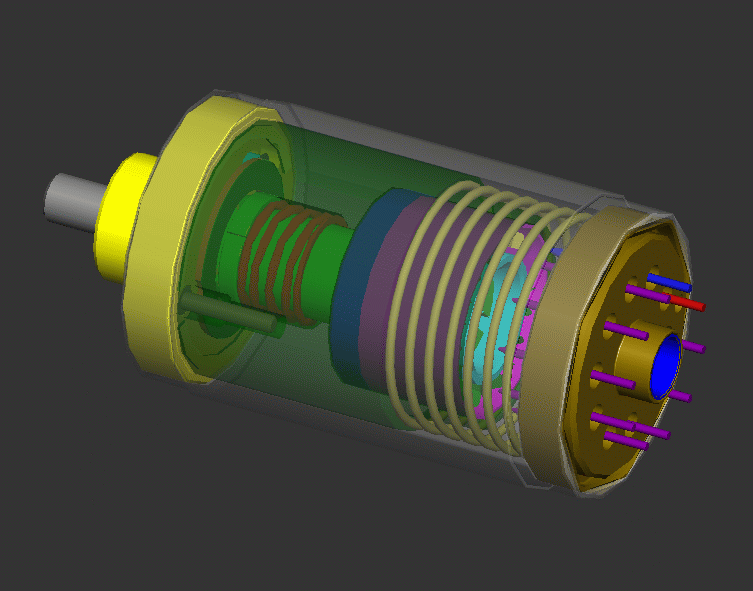
\includegraphics[width=0.5\textwidth]{Accelerometer.png}\end{center}
\caption{\label{fig:accelerometer}An accelerometer designed by the Archimedes Automated Assembly Planning Project at Sandia National Laboratory.}
\end{figure}
% image in the public domain, as it was created by the US government. See here for source: http://en.wikipedia.org/wiki/File:Accelerometer.png
Now, if we imagine this device in free-fall (don't drop your phones!), we can see that the spring will be at its rest position, while if the device was resting on the ground, the spring would be compressed under the weight of the test mass. Thus, an accelerometer measures acceleration relative to free-fall. In relativity theory, this acceleration is called \emph{proper acceleration}.
In Lab 2, you'll process the data from the accelerometer to measure footsteps. To get the absolute acceleration experienced by your phone, you will need to apply a low-pass filter to the acceleration data. Stay tuned for more information!
\section{Graphing}
For the next labs, it is enormously useful to be able to see how the accelerometer reacts when you manipulate the phone in various ways. We have provided an implementation of a line graph view that will display sets of data points. You will find {\tt LineGraphView.java} in the ``materials'' directory of the course repository. Figure \ref{fig:device-screenshot} shows what the graph view looks like. There is a bit of tearing in the screenshot of the graph because the process of taking a screenshot takes longer than one graph update.
\paragraph{Using the LineGraphView}
The following sample code shows how to set up the
{\tt LineGraphView} that we've provided. You are under
no obligation to use this code; you can provide your own,
if you want, or modify the code as you feel best, but chances are you
will just want to stick with the code we provided.
Note that you'll have to include an {\tt import} statement for this
class, since it belongs to the {\tt ca.uwaterloo.sensortoy}
package. Imports are like {\tt using} statements in C\#\footnote{\url{http://www.harding.edu/fmccown/java_csharp_comparison.html}}. Hitting Ctrl-Shift-O in Eclipse often fixes your imports.
\begin{lstlisting}{}
class MainActivity {
LineGraphView graph;
public void onCreate(Bundle savedInstanceState) {
// ... code was already here ...
LinearLayout layout = ((LinearLayout)findViewById(R.id.layout));
graph = new LineGraphView(getApplicationContext(),
100,
Arrays.asList("x", "y", "z"));
layout.addView(graph);
graph.setVisibility(View.VISIBLE);
// ... other code ...
}
}
\end{lstlisting}
Relevant parameters in the
constructor call are 100 and \verb+Arrays.asList("a", "b", "c")+. The 100 represents the number of samples to keep on the
t-axis. The syntax {\tt Arrays.asList("x", "y", "z")} is Java
shorthand for providing a list of labels for the graph.
The {\tt LineGraphView}'s constructor takes three parameters. The first is the application context. It is a special object that the view needs to know how to interact with the global state of the Android OS. The second parameter is an integer telling the {\tt LineGraphView} how many samples its X axis should be. The last parameter is an Object that implements Java's {\tt List} interface. This object should contain a list of strings that will be used as the labels of the different lines in the graph. Here is some sample code initialising a three-variable graph. It should go into the {\tt onCreate()} method of your {\tt Activity}.
Once you've created your view, you can start adding data to it. Use methods {\tt addPoint()} and {\tt purge()}. {\tt purge()} will clear the graph. {\tt addPoint()} takes either an array or {\tt List} of data points. The data must be in the same order as the labels that were passed into the constructor. We'll include an example of how to populate the graph below.
\paragraph{Integrating the {\tt LineGraphView}.} Now you have code to handle sensor changes. You can hook up the LineGraphView as follows.
\begin{lstlisting}{}
public void onSensorChanged(SensorEvent event) {
// ... other code ...
graph.addPoint(event.values);
// ... other code ...
}
\end{lstlisting}
\paragraph{Deliverable.} Plot the accelerometer data in graphical format.
%% \section{Create a system to transfer the collected data from the phone to your computer}
%\paragraph{File API}
%Android supports the standard Java file APIs. An important thing to keep in mind is that most phones have two kinds of memory. Internal memory that %is not accessible to the computer, and external flash memory that can be read when you connect to your computer. You can get a handle to the %external memory directory by calling {\tt getExternalFilesDir()} in your {\tt Activity} and passing null to it. You can then create a file in that %directory and write to it with a {\tt FileOutputStream}. You may also find the static method {\tt File.createTempFile()} useful.
%% Also, create a button which will clear the sensor history.
%% \paragraph{CSV files}
%% A Comma Separated Value file is a very simple file format for storing tabular data in a portable format. Every single spreadsheet program will open .csv files. The essence of a .csv is that you have data stored as text, and two characters are reserved as control characters. One character separates columns, and one separates rows. Usually, the column separator is the comma and the row separator is the carriage return.
%% For example, the .csv file:
%% \begin{lstlisting}[frame=trbl]{}
%% x,y,z
%% 1,2,3
%% 10,20,30
%% 0,2,5
%% \end{lstlisting}
%% would look like this when imported into a spreadsheet:
%% \begin{tabular}{|l|l|l|}
%% \hline
%% x&y&z \\
%% \hline
%% 1&2&3 \\
%% \hline
%% 10&20&30 \\
%% \hline
%% 0&2&5 \\
%% \hline
%% \end{tabular}
%% \paragraph{Deliverables.} Your solution must:
%% \begin{itemize}
%% \item include a button which saves historical sensor data to the phone's memory;
%% \item include a button which clears the log of historical sensor data.
%% \end{itemize}
\section{Test}
Your application should now display the current values of the sensors. You must display sensor values showing the three components of each sensor along with the lifetime maximum reading for these components. Also, you must display a graph of the accelerometer sensor readings over time. Your application should not crash or throw exceptions.
\section{Demonstration}
Once you are satisfied that your design and implementation are working correctly, arrange a demonstration with a teaching assistant. You will need to have the TA complete an assessment form. All of the members of your laboratory group must sign the completed assessment form. Your grade will be based on the results of the project demonstration at the end of the laboratory session and an evaluation of how well your code follows engineering design principles. (We will run plagiarism detection software on the source code, which may subsequently lower your grade and trigger a Policy 71 case. Don't plagiarize!)
\paragraph{Writing Good Code.} Your application must follow good engineering design principles. You should therefore avoid: unnecessary code duplication; excessive use of variables the state of which you keep synchronized manually; forgetting to deallocate (free up) resources like files you have requested from the Android OS; and any other such design failures that make your application difficult to maintain or that step on the toes of other applications you share the device with.
\section{Submission of project files}
Commit the {\tt Lab1\_SSS\_XX} files to your Subversion repository. The TAs will not mark labs that have not been submitted to SVN. The address is
\url{https://ecesvn.uwaterloo.ca/courses/ece155/w15/groups/group-NNN-MM}
Email Sanjay Singh if you can't commit to that address.
%% \todo{Do we want to evaluate their code for maintainability / good design / etc?, also, what is the best way to evaluate code? On site or afterwards? During the demo, students can defend their design, but afterwards, we can give better feedback.}
\section{Too Long; Did Not Read}
If you just want to cut to the chase and get an exact listing of what to do, check the lab 1 assessment form and you will see exactly what we are looking for in the deliverables for this lab.
\end{document}
